\PassOptionsToPackage{unicode=true}{hyperref} % options for packages loaded elsewhere
\PassOptionsToPackage{hyphens}{url}
%
\documentclass[]{article}
\usepackage{lmodern}
\usepackage{amssymb,amsmath}
\usepackage{ifxetex,ifluatex}
\usepackage{fixltx2e} % provides \textsubscript
\ifnum 0\ifxetex 1\fi\ifluatex 1\fi=0 % if pdftex
  \usepackage[T1]{fontenc}
  \usepackage[utf8]{inputenc}
  \usepackage{textcomp} % provides euro and other symbols
\else % if luatex or xelatex
  \usepackage{unicode-math}
  \defaultfontfeatures{Ligatures=TeX,Scale=MatchLowercase}
\fi
% use upquote if available, for straight quotes in verbatim environments
\IfFileExists{upquote.sty}{\usepackage{upquote}}{}
% use microtype if available
\IfFileExists{microtype.sty}{%
\usepackage[]{microtype}
\UseMicrotypeSet[protrusion]{basicmath} % disable protrusion for tt fonts
}{}
\IfFileExists{parskip.sty}{%
\usepackage{parskip}
}{% else
\setlength{\parindent}{0pt}
\setlength{\parskip}{6pt plus 2pt minus 1pt}
}
\usepackage{hyperref}
\hypersetup{
            pdftitle={High(er) order epistasis and strength of drift},
            pdfauthor={Florian Labourel},
            pdfborder={0 0 0},
            breaklinks=true}
\urlstyle{same}  % don't use monospace font for urls
\usepackage[margin=1in]{geometry}
\usepackage{color}
\usepackage{fancyvrb}
\newcommand{\VerbBar}{|}
\newcommand{\VERB}{\Verb[commandchars=\\\{\}]}
\DefineVerbatimEnvironment{Highlighting}{Verbatim}{commandchars=\\\{\}}
% Add ',fontsize=\small' for more characters per line
\usepackage{framed}
\definecolor{shadecolor}{RGB}{248,248,248}
\newenvironment{Shaded}{\begin{snugshade}}{\end{snugshade}}
\newcommand{\AlertTok}[1]{\textcolor[rgb]{0.94,0.16,0.16}{#1}}
\newcommand{\AnnotationTok}[1]{\textcolor[rgb]{0.56,0.35,0.01}{\textbf{\textit{#1}}}}
\newcommand{\AttributeTok}[1]{\textcolor[rgb]{0.77,0.63,0.00}{#1}}
\newcommand{\BaseNTok}[1]{\textcolor[rgb]{0.00,0.00,0.81}{#1}}
\newcommand{\BuiltInTok}[1]{#1}
\newcommand{\CharTok}[1]{\textcolor[rgb]{0.31,0.60,0.02}{#1}}
\newcommand{\CommentTok}[1]{\textcolor[rgb]{0.56,0.35,0.01}{\textit{#1}}}
\newcommand{\CommentVarTok}[1]{\textcolor[rgb]{0.56,0.35,0.01}{\textbf{\textit{#1}}}}
\newcommand{\ConstantTok}[1]{\textcolor[rgb]{0.00,0.00,0.00}{#1}}
\newcommand{\ControlFlowTok}[1]{\textcolor[rgb]{0.13,0.29,0.53}{\textbf{#1}}}
\newcommand{\DataTypeTok}[1]{\textcolor[rgb]{0.13,0.29,0.53}{#1}}
\newcommand{\DecValTok}[1]{\textcolor[rgb]{0.00,0.00,0.81}{#1}}
\newcommand{\DocumentationTok}[1]{\textcolor[rgb]{0.56,0.35,0.01}{\textbf{\textit{#1}}}}
\newcommand{\ErrorTok}[1]{\textcolor[rgb]{0.64,0.00,0.00}{\textbf{#1}}}
\newcommand{\ExtensionTok}[1]{#1}
\newcommand{\FloatTok}[1]{\textcolor[rgb]{0.00,0.00,0.81}{#1}}
\newcommand{\FunctionTok}[1]{\textcolor[rgb]{0.00,0.00,0.00}{#1}}
\newcommand{\ImportTok}[1]{#1}
\newcommand{\InformationTok}[1]{\textcolor[rgb]{0.56,0.35,0.01}{\textbf{\textit{#1}}}}
\newcommand{\KeywordTok}[1]{\textcolor[rgb]{0.13,0.29,0.53}{\textbf{#1}}}
\newcommand{\NormalTok}[1]{#1}
\newcommand{\OperatorTok}[1]{\textcolor[rgb]{0.81,0.36,0.00}{\textbf{#1}}}
\newcommand{\OtherTok}[1]{\textcolor[rgb]{0.56,0.35,0.01}{#1}}
\newcommand{\PreprocessorTok}[1]{\textcolor[rgb]{0.56,0.35,0.01}{\textit{#1}}}
\newcommand{\RegionMarkerTok}[1]{#1}
\newcommand{\SpecialCharTok}[1]{\textcolor[rgb]{0.00,0.00,0.00}{#1}}
\newcommand{\SpecialStringTok}[1]{\textcolor[rgb]{0.31,0.60,0.02}{#1}}
\newcommand{\StringTok}[1]{\textcolor[rgb]{0.31,0.60,0.02}{#1}}
\newcommand{\VariableTok}[1]{\textcolor[rgb]{0.00,0.00,0.00}{#1}}
\newcommand{\VerbatimStringTok}[1]{\textcolor[rgb]{0.31,0.60,0.02}{#1}}
\newcommand{\WarningTok}[1]{\textcolor[rgb]{0.56,0.35,0.01}{\textbf{\textit{#1}}}}
\usepackage{graphicx,grffile}
\makeatletter
\def\maxwidth{\ifdim\Gin@nat@width>\linewidth\linewidth\else\Gin@nat@width\fi}
\def\maxheight{\ifdim\Gin@nat@height>\textheight\textheight\else\Gin@nat@height\fi}
\makeatother
% Scale images if necessary, so that they will not overflow the page
% margins by default, and it is still possible to overwrite the defaults
% using explicit options in \includegraphics[width, height, ...]{}
\setkeys{Gin}{width=\maxwidth,height=\maxheight,keepaspectratio}
\setlength{\emergencystretch}{3em}  % prevent overfull lines
\providecommand{\tightlist}{%
  \setlength{\itemsep}{0pt}\setlength{\parskip}{0pt}}
\setcounter{secnumdepth}{0}
% Redefines (sub)paragraphs to behave more like sections
\ifx\paragraph\undefined\else
\let\oldparagraph\paragraph
\renewcommand{\paragraph}[1]{\oldparagraph{#1}\mbox{}}
\fi
\ifx\subparagraph\undefined\else
\let\oldsubparagraph\subparagraph
\renewcommand{\subparagraph}[1]{\oldsubparagraph{#1}\mbox{}}
\fi

% set default figure placement to htbp
\makeatletter
\def\fps@figure{htbp}
\makeatother

\usepackage{amsmath}

\title{High(er) order epistasis and strength of drift}
\author{Florian Labourel}
\date{}

\begin{document}
\maketitle

\hypertarget{why-on-earth-should-we-worry-about-effects-of-epistasis-an-idea-coming-from-cellular-models-of-fitness}{%
\subsection{Why on earth should we worry about effects of epistasis: an
idea coming from cellular models of
fitness?}\label{why-on-earth-should-we-worry-about-effects-of-epistasis-an-idea-coming-from-cellular-models-of-fitness}}

Enzyme-substrate reactions (see top panel of the figure below) rely on
the binding (at a rate \(k_f\)) between these two molecules, that can
then either dissociate (at a rate \(k_r\), these pointless meetings
decrease the rate of the reaction) or undergo the process of catalysis
(at a rate \(k_{cat}\)) that releases the enzyme and a newly formed
product. Therefore, Evolution should in first approach maximise both
\(k_f\) and \(k_{cat}\). The process can be described through
Michaelis-Menten equation, where the flux at steady-state is given by
the following equation:

\begin{equation}
v=k_{cat}.[E_\text{tot}].\frac{[S]}{K_\text{M}+[S]},
\label{EquiBHsimp}
\end{equation} \noindent under the assumption that the concentration
\([S]\) is approximately constant and that of \([ES]\) is at equilibrium
%\citep{MichaelisMenten1913, Briggs25}. In this equation,
\(K_M=\dfrac{k_\text{r}+k_\text{cat}}{k_\text{f}}\) represents an
affinity term: the lower the better.

In this framework, it is possible to study the kinetic efficiency of
enzymes. When we do so, the results is quite unexpected: enzymes seem to
belong to a zoo where variation is the rule (see three panels below).
One may then wonder why most enzymes are so far from their kinetic
optimum (and so different one from another).

\begin{figure}

{\centering 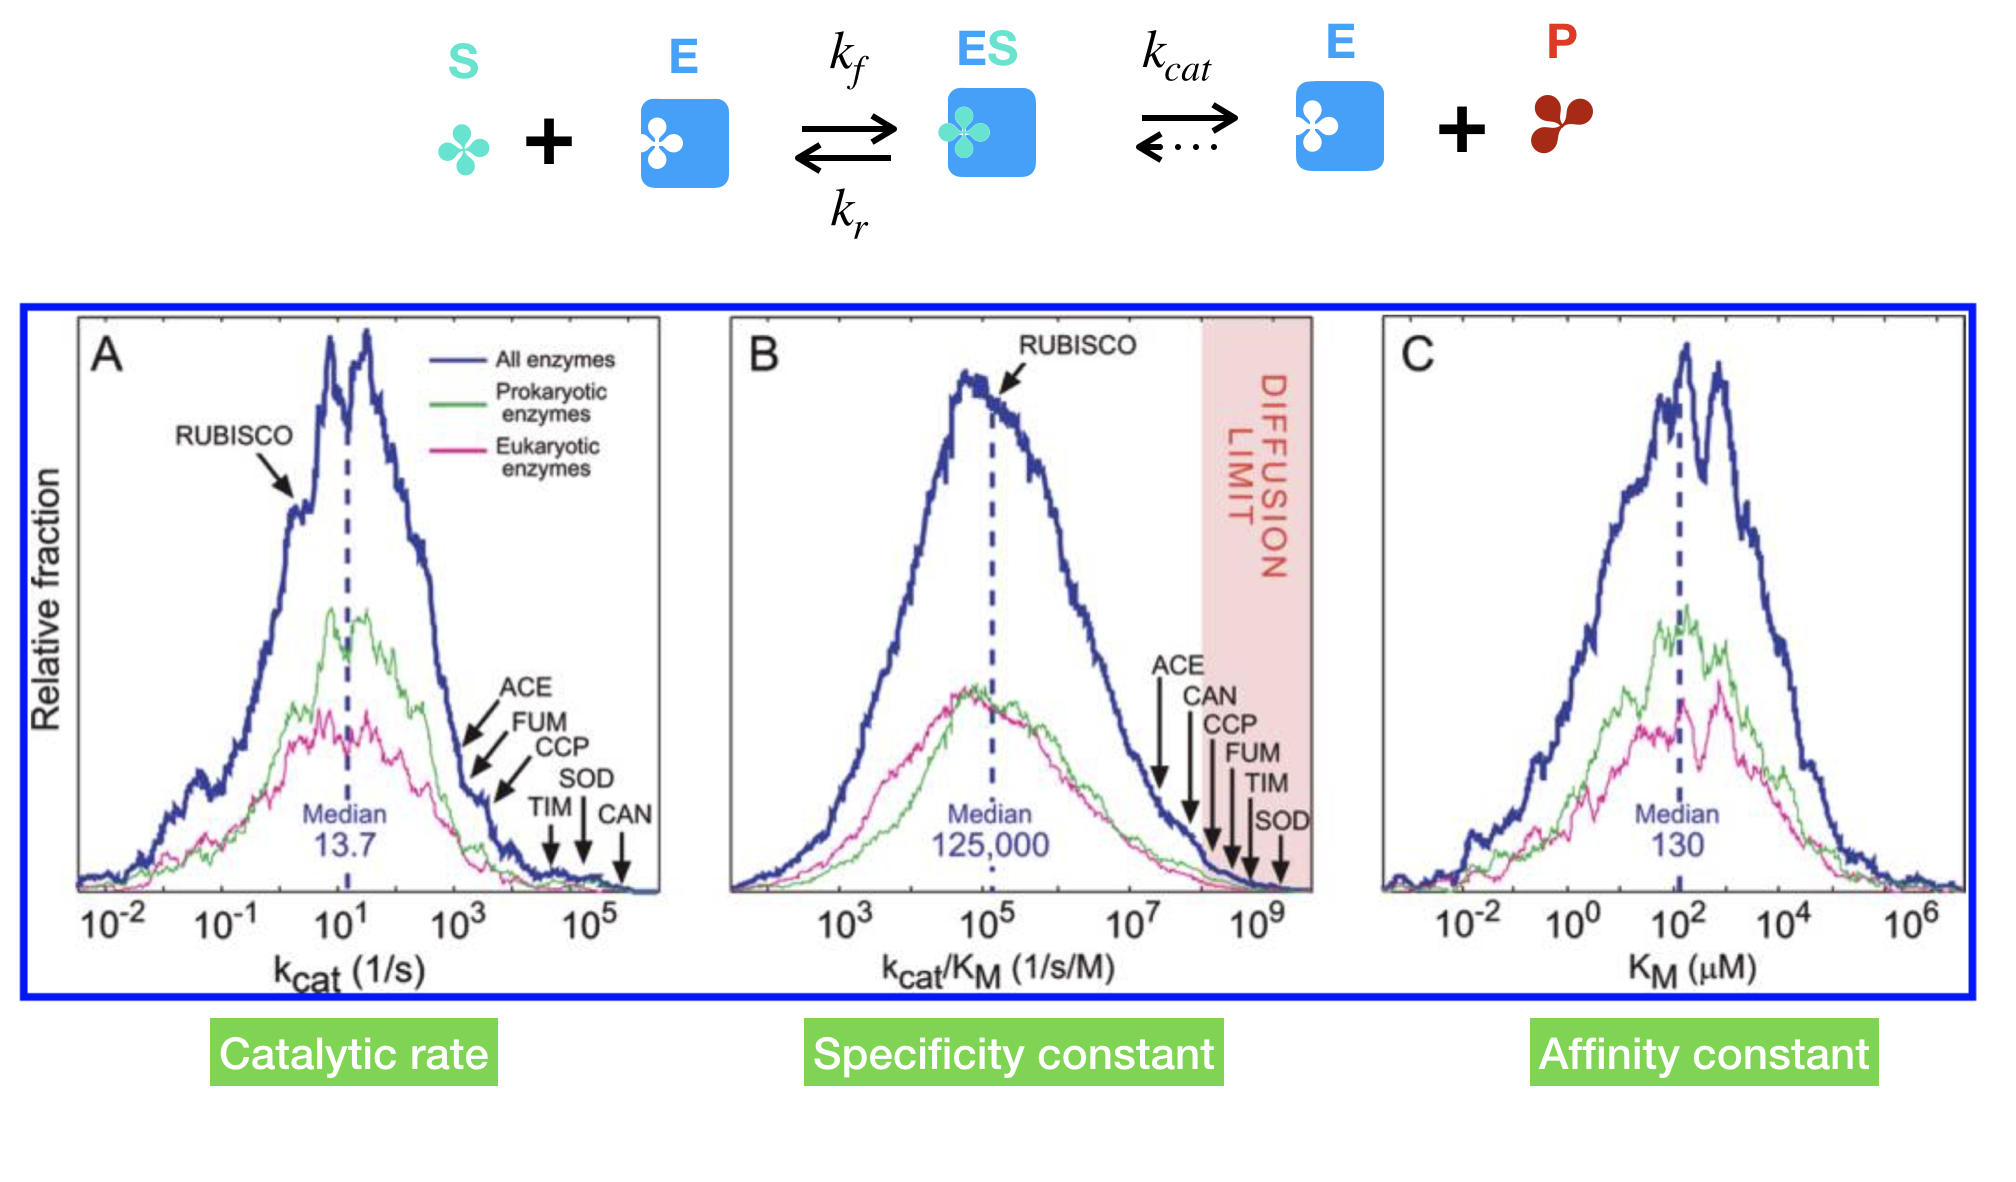
\includegraphics[width=1\linewidth]{Enzyme_zoo} 

}

\caption{Enzyme zoo: widespread (and yet to be explained) variation in enzyme kinetics (source: Bar-Even et al., 2011)}\label{fig:enzoo}
\end{figure}

\newpage

When introducing more parameters, enzymes generally evolve on
plateau-like fitness landscapes (results from many diferent theories:
control of flux (Kacser and Burns, 73; Rapoport and Heinrich, 74;
Dykhuizen, 88), protein stability, metabolix flux analysis; see right
panel on the following figure); nonetheless, we have shown that several
parameters are involved in the fitness landscapes on which enzymes
evolve, one of which is the level of the flux an enzyme has to sustain:

\begin{figure}

{\centering 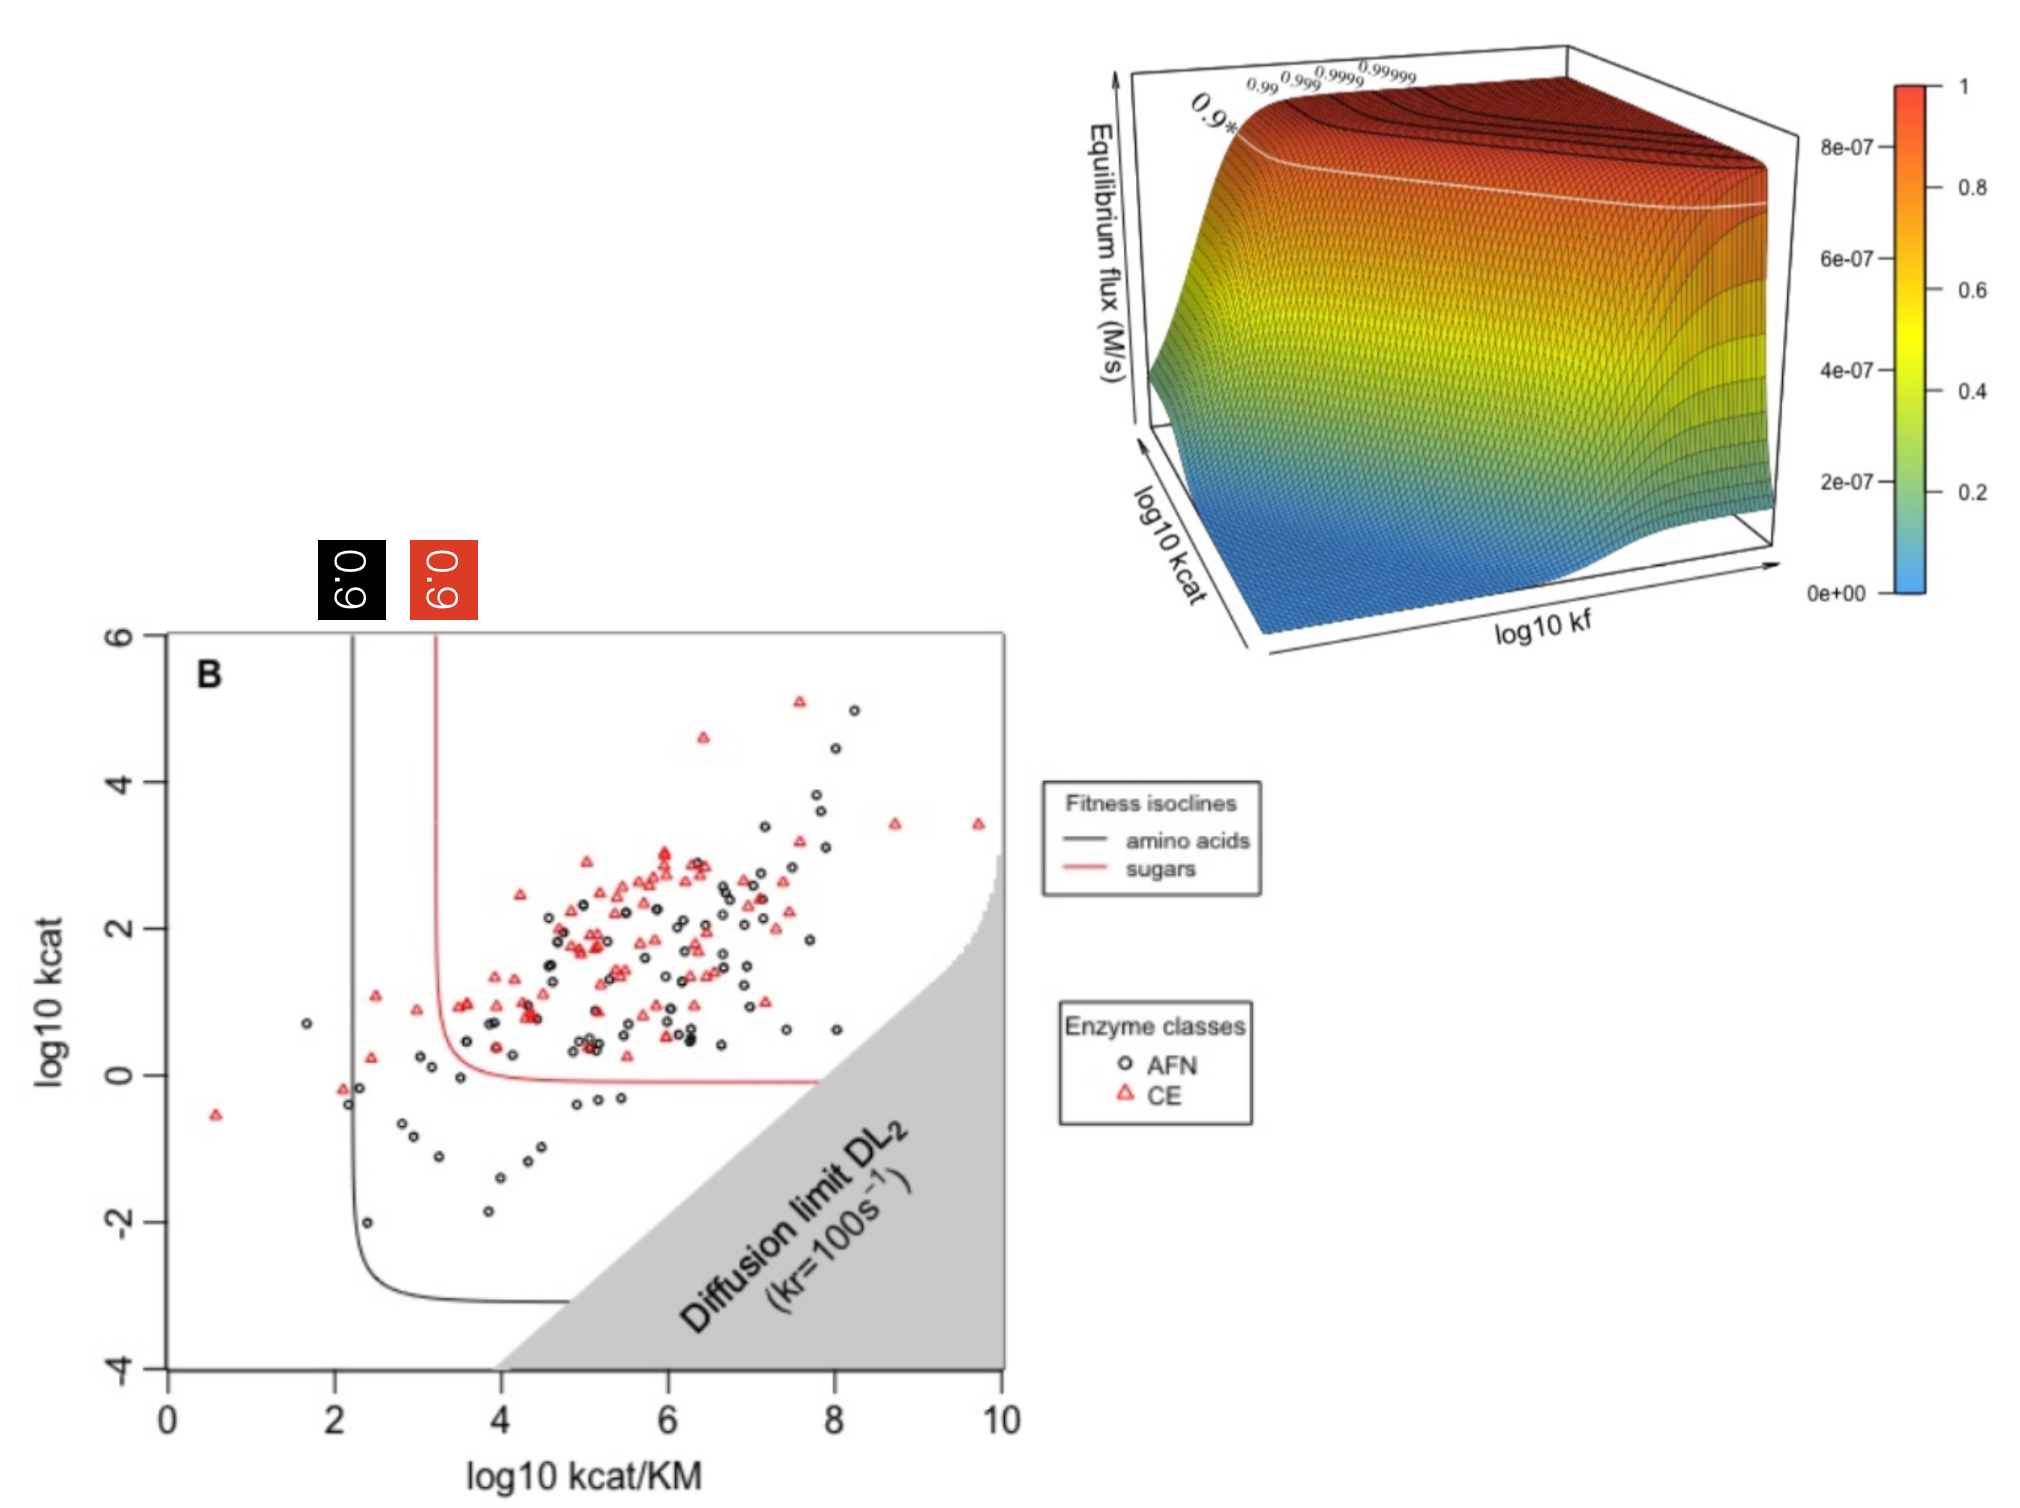
\includegraphics[width=1\linewidth]{Enzyme_zoo_explanation} 

}

\caption{Enzyme zoo, some pieces of explanation: the levels of flux in a given pathway}\label{fig:enzooexplain}
\end{figure}

But still, enzymes should be far more efficient and \(N_e\) should be a
(if not the) major driver of their evolution as population genetics
assuming realistic mutational landscapes shown:

\begin{figure}

{\centering 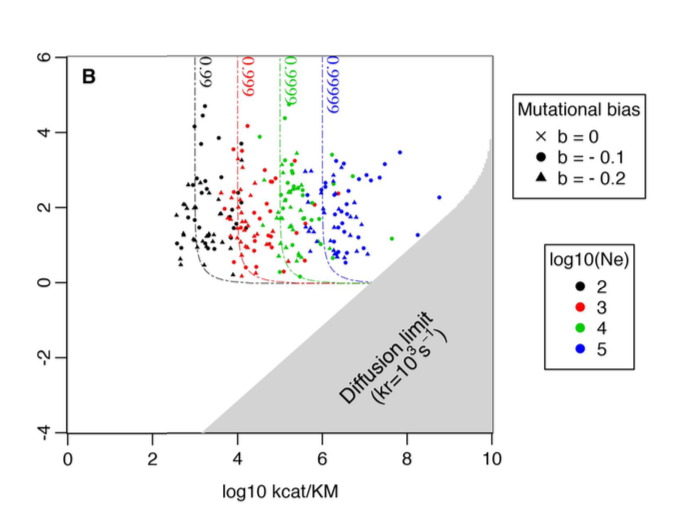
\includegraphics[width=0.7\linewidth]{Enzyme_simulated} 

}

\caption{Enzyme zoo: the paradox of }\label{fig:enzsim}
\end{figure}

One explanation of why Evolution underperforms (if it is the case - some
biophysicists think that cells may be tuned to sustain specific flux
levels rather than ; others think that some physics constraints may be
impossible to escape such that they disable Evolution to act as it
should be) is the existence of epistasis between enzymes.

\newpage

\hypertarget{brief-recall-about-epistasis}{%
\subsection{Brief recall about
epistasis}\label{brief-recall-about-epistasis}}

Epistasis: process by which the effect of the mutation is dependent on
the genetic background in which it appears. In other words, it is the
part of variance that cannot be explained by effects of additivity or
dominance. When two mutations are present, there is a departure from the
prediction of additivity (additivity: first case in the figure below;
different kind of epistasis are shown next to it).

\begin{figure}

{\centering 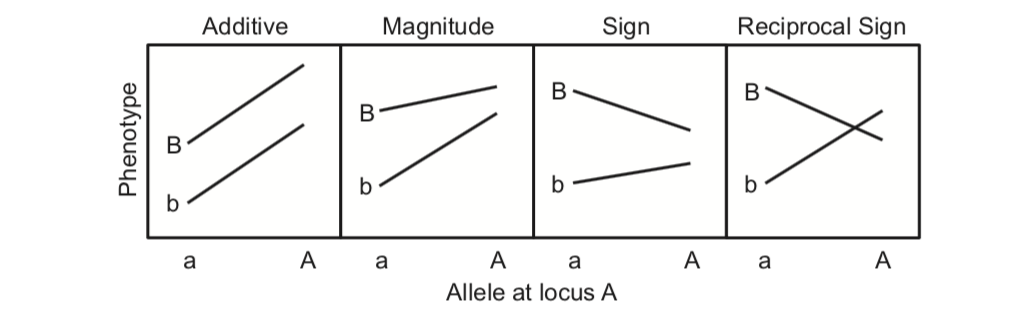
\includegraphics[width=1\linewidth]{Epistasis_description} 

}

\caption{Weinreich definition: epistasis (three panels on the right) is a measure of our surprise}\label{fig:epi_gen}
\end{figure}

Epistasis has long been discussed in the case of the fitness landscape
analogy that describes Evolution as a climbing process that may or may
not be deterministic. More particularly, it has been demonstrated that
in a constant environment, where organisms can be represented on one and
only one fitness landscape, rugged landscape can arise if and only if
there is some reciprocal sign epistasis, which produces valleys (and
potentially ruggedness) separating different peaks that opens the door
to evolutionary contingency.

\begin{figure}

{\centering 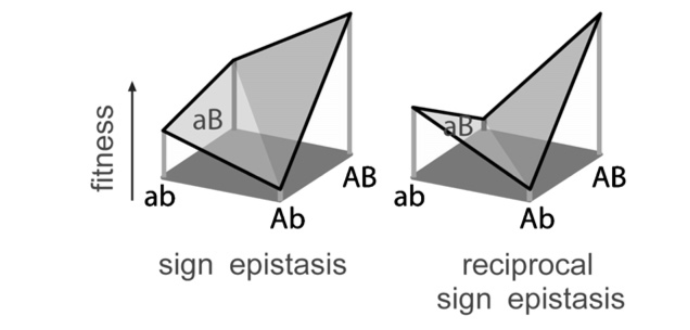
\includegraphics[width=1\linewidth]{Sign_epistasis&fitnessPeaks} 

}

\caption{Epistasis and fitness}\label{fig:epifit}
\end{figure}

The idea here is to study the case of complementary epistasis when it
involves a large number of loci/genes/modules all needed in order to
perform a given task at a given level (eg. enzymes involved in a
metabolic pathway: if one is worse than the others, the flux is
decreased; different cellular pathways: producing a lot of a given
amino-acid may be useless if ribosomes are too slow to use them, or if
nucleotids are produced at a slower pace (relatively to that of the
aforementionned amino-acid; a very efficient stomach might be useless if
the gut or the liver underperforms).

\hypertarget{the-particular-case-of-complementary-epistasis}{%
\subsection{The particular case of complementary
epistasis}\label{the-particular-case-of-complementary-epistasis}}

Complementary epistasis : both genes are needed to give rise to a new
phenotype as shown below (A and B can only produce their effect if they
are expressed together; otherwise, none of them has any effect at all
(to study it in a generic case) - neutral mutation). This is well-known
for pigment coloration in corn, for instance, where changing the color
relies on the presence of two mutations (in some cases).

\begin{figure}

{\centering 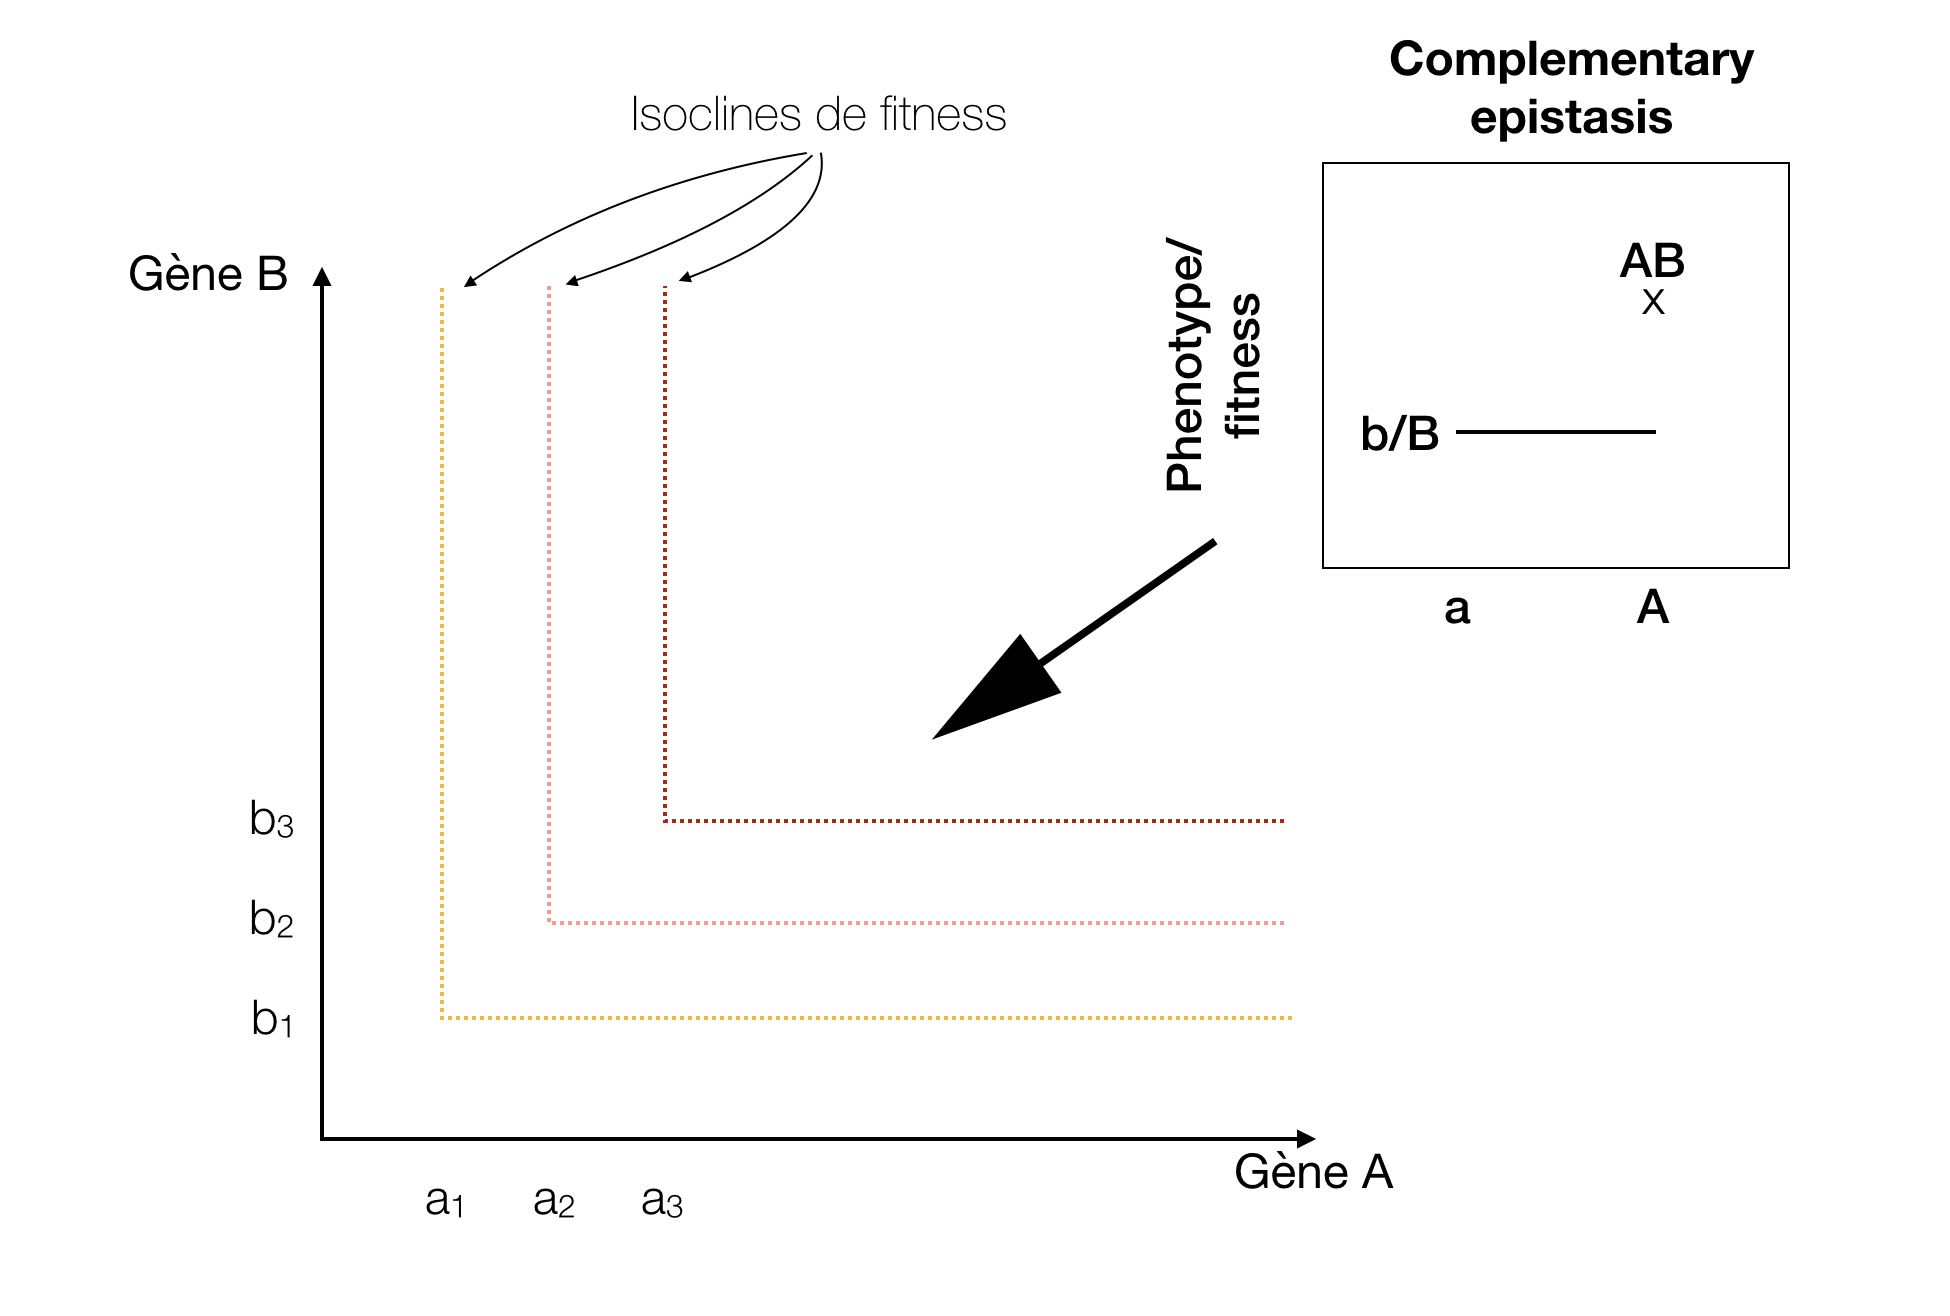
\includegraphics[width=1\linewidth]{Complementary_epistasis} 

}

\caption{Complementary epistasis and fitness isoclines}\label{fig:compepi}
\end{figure}

Under such assumptions, increasing fitness relies on a two-step process:
first, a dormant advantageous mutation has to evolve through drift as
its effect on fitness is perfectly neutral. Only then fitness can be
improved thanks to a second advantageous mutation occuring on the
complementary gene.

\begin{figure}

{\centering 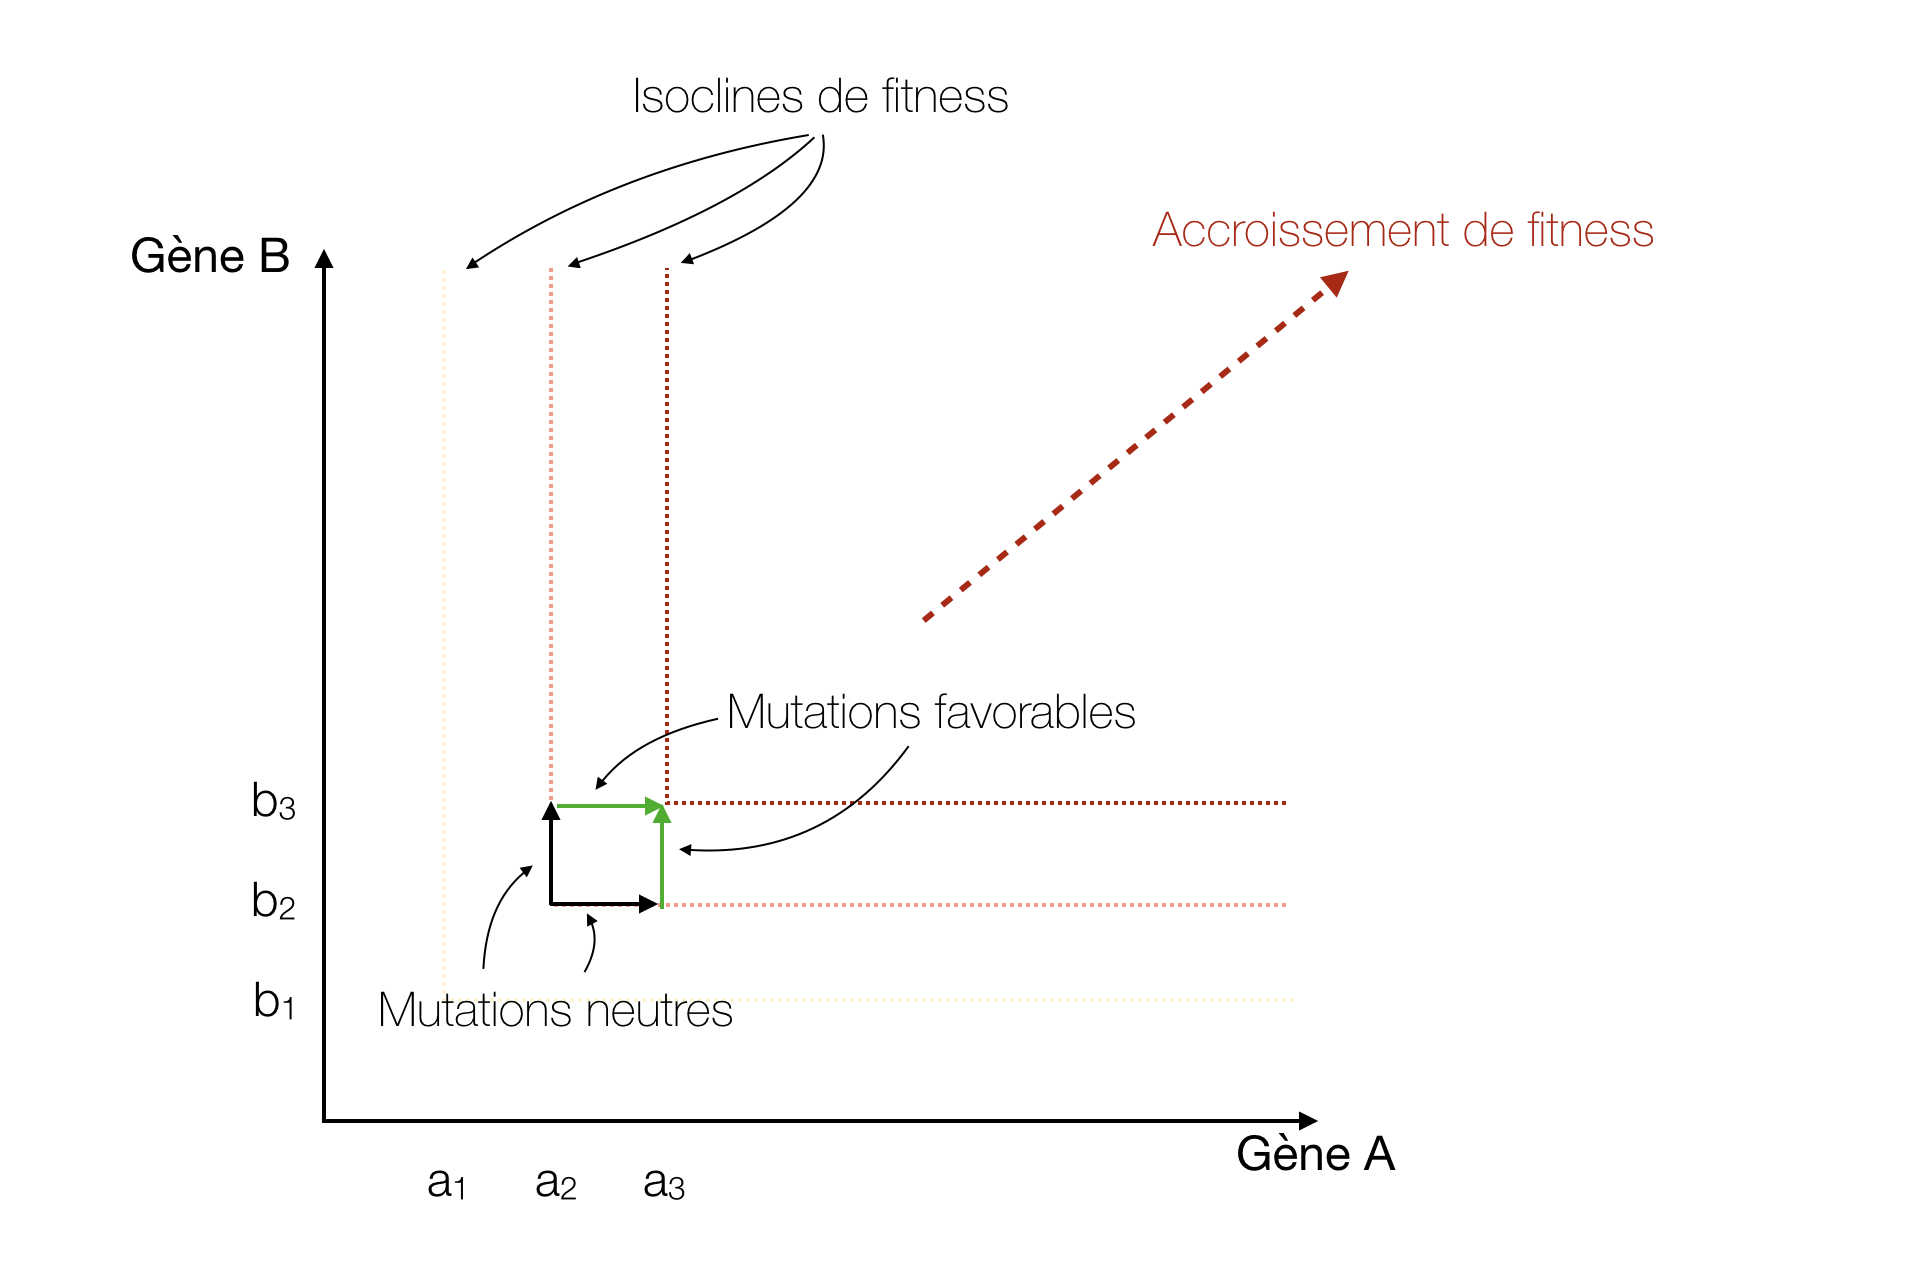
\includegraphics[width=1\linewidth]{Evo_Complementary_epistasis} 

}

\caption{Complementary epistasis and evolutionary trajectories: only the last beneficial mutation gives an extra fitness to its carrier}\label{fig:trajcompepi}
\end{figure}

As it is cumbersome to draw hypervolume with many dimensions, we got
focused on the simplistic case of two complementary genes. One way then
wonder what would happen if higher order epistasis comes into play.

High(er) order epistasis : epistatic interactions depend on a high
number of interactions (\textgreater{}\textgreater{}2 genes)

\hypertarget{first-studies-on-the-influence-of-the-combination-of-drift-and-higher-order-epistasis}{%
\subsection{First studies on the influence of the combination of drift
and high(er) order
epistasis}\label{first-studies-on-the-influence-of-the-combination-of-drift-and-higher-order-epistasis}}

Some authors have recently raised the need to address this process (in
the case of enzyme turn-over numbers \(k_{cat}\)s for instance). In
their model, the fitness of cells result from the complex combination of
thousands of enzymes whose \(k_{cat}\)s can undergo mutations. Mutation
fixation of one variant is computed by a random draw from a binomial
distribution with (Kimura:61)'s formula for fixation probability.

\begin{center}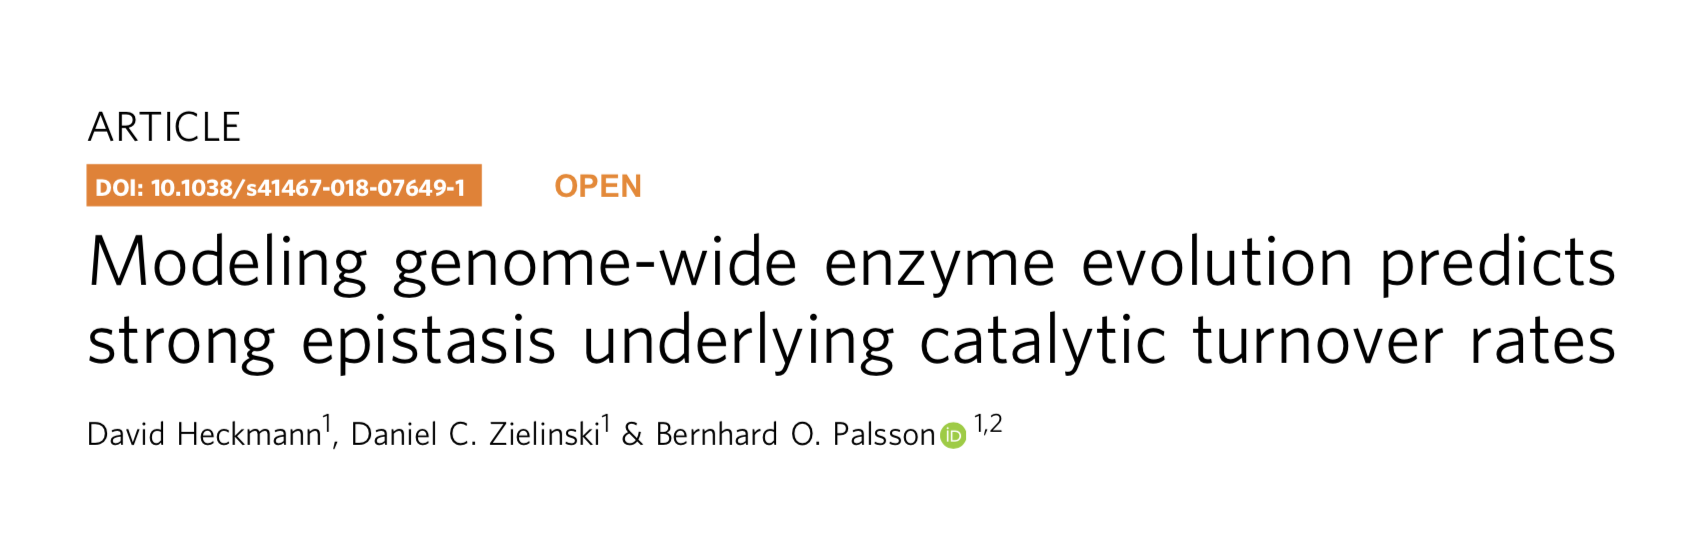
\includegraphics[width=1\linewidth]{Heckmannetal..png} \end{center}

And they have shown that it may account for the wide variability among
enzymes efficiency within an organism, as their outcomes recnstruct most
of this variability:

\begin{figure}

{\centering 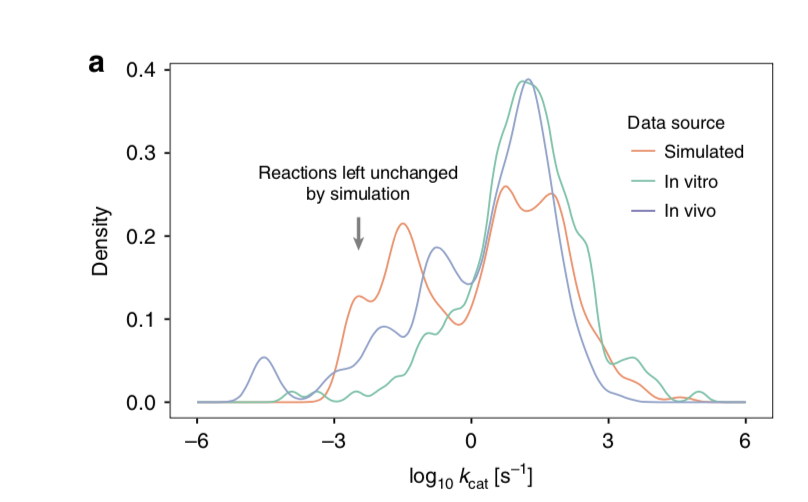
\includegraphics[width=1\linewidth]{Heckmann_comparison} 

}

\caption{Turn-over numbers hit a ceiling in the different pathways}\label{fig:simkcat}
\end{figure}

Here, the authors fixed some enzymes to moderate values for there seems
to exist an upper-limit to some of them (dubious to me in first
approach, see their explanations in the quotation reported below). This
strong assumption limits the interest of their findings to me and might
explain alone that enzymes are stuck to low values in their model.

\begin{figure}

{\centering 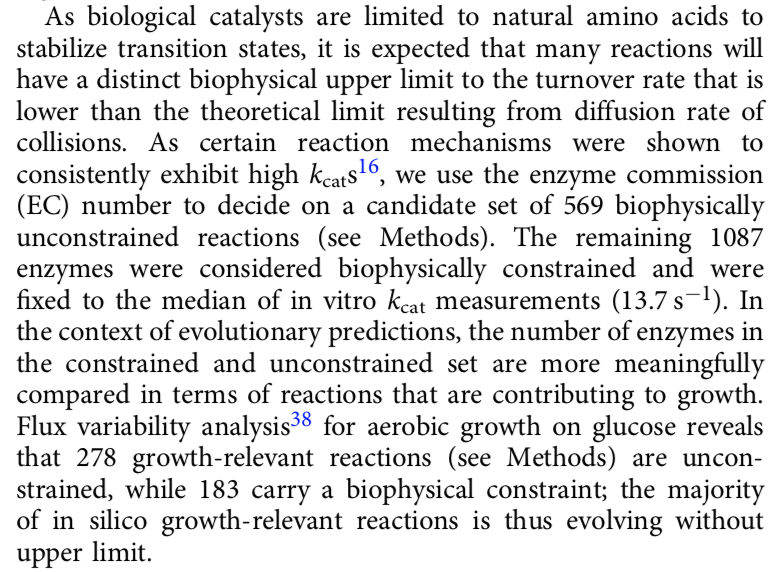
\includegraphics[width=0.5\linewidth]{Constrained_enzymes_Heckmann} 

}

\caption{Explanations about constrained enzymes from Heckamnn et al.(2019)}\label{fig:constenz}
\end{figure}

The aim of the present document is to test what would happen when an
enzyme's fitness depends on its genetic background in a complementary
fashion (and in other cases for which this framework could make some
sense) and, more specifically, how biased mutations - towards
deleterious effects - would affect the evolutionary process.

\hypertarget{a-toy-model-to-test-the-effect-within-a-general-framework}{%
\subsection{A toy model to test the effect within a general
framework}\label{a-toy-model-to-test-the-effect-within-a-general-framework}}

\begin{enumerate}
\def\labelenumi{\arabic{enumi})}
\item
  Fitness is determined by the selective value of the worst enzyme of an
  organism. Eg. set of 3 enzymes with selective value (0.9,0.95,1)
  yields a fitness of 0.9
\item
  A time-step corresponds to a mutational event conerning one
  gene/module of the set. Each mutation can then invade the population
  or be removed during the timestep (no polymorphism occurs here, to
  stay as simple as possible). Its probability of fixation depends on
  the gain of fitness (to the haploid organism) it provides, according
  to Kimura equation (Kimura,1961):
\end{enumerate}

\begin{Shaded}
\begin{Highlighting}[]
\CommentTok{#Fixation probability}
\NormalTok{u_exact<-}\ControlFlowTok{function}\NormalTok{(s,Ne,p)\{}
  \KeywordTok{return}\NormalTok{((}\DecValTok{1}\OperatorTok{-}\KeywordTok{exp}\NormalTok{(}\OperatorTok{-}\DecValTok{2}\OperatorTok{*}\NormalTok{Ne}\OperatorTok{*}\NormalTok{s}\OperatorTok{*}\NormalTok{p))}\OperatorTok{/}\NormalTok{(}\DecValTok{1}\OperatorTok{-}\KeywordTok{exp}\NormalTok{(}\OperatorTok{-}\DecValTok{2}\OperatorTok{*}\NormalTok{Ne}\OperatorTok{*}\NormalTok{s)))}
\NormalTok{\}}
\end{Highlighting}
\end{Shaded}

Note: If a mutation improves an enzyme that is not the worst one, its
probability of fixation is that of a neutral mutation.

\begin{enumerate}
\def\labelenumi{\arabic{enumi})}
\setcounter{enumi}{2}
\tightlist
\item
  Mutations are drawn randomly from beta distributions with different
  properties (4 cases), as shown below:
\end{enumerate}

\begin{figure}

{\centering \includegraphics[width=0.9\linewidth]{1.Drift-Epistasis_files/figure-latex/unnamed-chunk-2-1} 

}

\caption{Distribution of fitness effects of mutations in the different cases}\label{fig:unnamed-chunk-2}
\end{figure}

Note: the distribution of fitness effects is dependent on the present
value of the gene (latent) fitness. In other words, a better enzyme has
a higher mutational average fitness (eg. an enzyme with fitness 1
(maximum) have more mutations that yield a fitness f=1 than en enzyme
with fitness 0.5).

\begin{enumerate}
\def\labelenumi{\arabic{enumi})}
\setcounter{enumi}{3}
\tightlist
\item
  The initial fitness value of each enzyme/gene/locus is set to the
  rather high value of \(0.9\), sufficiently far away from high values
  to avoid boundary conditions problems (unclear why it is a problem at
  this point, may be creating some nearly absorbing states). \#, the
  (Kimura) expected outcome of Evolution when there is a high mutational
  bias towards deleterious effects.
\end{enumerate}

\hypertarget{results-of-the-toy-model}{%
\subsection{Results of the toy model}\label{results-of-the-toy-model}}

Simulations are ran over an average of \(100N_e\) mutational events
occuring on each module, with 30 replicates for each set of parameters.
The first case considers here considers that \(N_e=10\), for which we
report fitness outcomes when the evolutionary steady-state has been
reached:

\begin{figure}

{\centering \includegraphics[width=1\linewidth]{1.Drift-Epistasis_files/figure-latex/hoe_out_10-1} 

}

\caption{Very preliminary simulation outcomes ($N_e=10$) : effect of complementary epistasis on fitness at evolutionary steady-state}\label{fig:hoe_out_10}
\end{figure}

The following reults display what happens for fitness when \(N_e=100\):

\begin{figure}

{\centering \includegraphics[width=1\linewidth]{1.Drift-Epistasis_files/figure-latex/hoe_out_100-1} 

}

\caption{Very preliminary simulation outcomes ($N_e=100$) : effect of complementary epistasis on fitness at evolutionary steady-state}\label{fig:hoe_out_100}
\end{figure}

The following reults display what happens for fitness when \(N_e=1000\):

\begin{figure}

{\centering \includegraphics[width=1\linewidth]{1.Drift-Epistasis_files/figure-latex/hoe_out_1000-1} 

}

\caption{Very preliminary simulation outcomes ($N_e=1000$) : effect of complementary epistasis on fitness at evolutionary steady-state}\label{fig:hoe_out_1000}
\end{figure}

One limit of these toy models lies in the choice of the distribution,
which may trap the fitness in absorbing states (at very low values or
very high values), especially when \(N_e\) increases, as very few
mutations of the neutral area are sampled. Note that for the last
results, the scale was adjusted in the bottom panels to facilitate their
visualization.

What one can see is that outcomes are largely dependent on both the
fitness effect distribution and the amount of complementary
modules/genes (locus?) such that this process may help explain why most
mutations are evolving under neutral evolution even if they might be
necessary pieces to increase fitness. More importantly, it might help
reconcile the paradox between the fact that many genes seem to evolve
under neutrality while these genes still lie far from their theoretical
optimum (eg. of enzymes above).

\end{document}
